% 第3章第4节：二部图匹配（问题；与单位容量最大流的对应；匈牙利算法与分层改进；结果检验）。

\section{二部图匹配}
\label{sec:graph-matching}

把若干任务分给若干名人员，每人至多接一项任务，每项任务至多由一人负责，并且只有具备资格的人才能接相应的任务。我们要在允许的“人员—任务”配对中选出一组，任何人员或任务都不出现在两个配对里，使配对数量最多。

每人、每项任务至多用一次，与每条弧至多通过一单位流量是同一种限制，所以这个问题就是容量都为$1$的最大流。第~\ref{sec:graph-max-flow}节的残量路径落到二部图上，成为新旧配对交替的路径，沿它改配能多配一对；匈牙利算法直接记录配对，逐个为人员寻找这样的路径。

\subsection{二部图匹配问题}
\label{sec:graph-opt-match-problem}

人员与任务分属两类，资格关系只跨类连接。若无向图的顶点集能分成不相交的两部分$L$与$R$，使每条边恰有一个端点在$L$、另一个端点在$R$，就称它为\term{二部图}（bipartite graph），记作$\mathcal G=(L\cup R,E)$，并称$L$为左侧、$R$为右侧。边$\{u,w\}$（$u\in L$，$w\in R$）简记为$(u,w)$，称为允许边。一组配对合法，是指选出的边两两没有公共端点。

\begin{definition}[匹配]
\label{def:graph-opt-matching}
图$\mathcal G=(V,E)$中两两没有公共端点的边组成的集合$M\subseteq E$称为一个\term{匹配}（matching）。若$(u,w)\in M$，称$u$与$w$被$M$匹配，互为\emph{伙伴}；不被任何匹配边关联的顶点称为自由顶点。边数最多的匹配称为\term{最大匹配}（maximum matching），没有自由顶点的匹配称为\term{完美匹配}（perfect matching）。不能再加入任何一条边而仍为匹配的$M$称为\term{极大匹配}（maximal matching）。
\end{definition}

最大匹配一定是极大匹配，反之不然。设左侧为$a,b$，右侧为任务$1,2$，允许边为$(a,1)$、$(a,2)$、$(b,1)$，如图~\ref{fig:graph-opt-match-maximal-maximum}。若先选$(a,1)$，另两条边都与它共享端点，无法再加，所以$\{(a,1)\}$是极大匹配；可是$\{(a,2),(b,1)\}$有两条边，是最大匹配，也是完美匹配。从前者到后者不能继续加边，只能把$a$改派到任务$2$，腾出任务$1$给$b$。逐条贪心加边可能停在这样的结果上，改进必须允许重排已有的配对。

\begin{figure}[!htb]
  \centering
  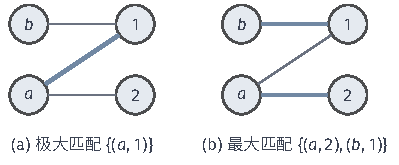
\includegraphics[width=67.515mm]{figures/01-basic-mathematics/04-graphs/tikz/c3-match-maximal-maximum/figure.pdf}
  \caption{极大匹配与最大匹配。细线为允许边，粗蓝线为匹配边。(a)极大匹配$\{(a,1)\}$；(b)最大匹配$\{(a,2),(b,1)\}$，由(a)到(b)须改动已有配对。}
  \label{fig:graph-opt-match-maximal-maximum}
\end{figure}

本节只最大化配对数$|M|$，边上没有成本；成本问题留到第~\ref{sec:graph-assignment}节。两侧大小可以不同，最大匹配至多有$\min\{|L|,|R|\}$条边，但未必达到：若两名人员都只会同一项任务，至多一人能配上。后面的构造利用给定的两侧划分；含奇数长环（如三角形）的一般图无法这样划分，不能直接套用。记$n=|L|+|R|$，$m=|E|$。

\subsection{匹配与最大流的对应}
\label{sec:graph-opt-match-alternating}

由二部图构造流网络：增加源点$s$与汇点$t$，从$s$向每个$u\in L$连弧，把每条允许边$(u,w)$改为弧$u\to w$，再从每个$w\in R$向$t$连弧，所有容量都为$1$，如图~\ref{fig:graph-opt-match-flow-network}。

给定匹配$M$，沿每条匹配边对应的路线$s\to u\to w\to t$各送一单位，得到流值为$|M|$的整数流。反过来，整数流$\bm x$在每条弧上只取$0$或$1$。左侧顶点$u$只有一条容量为$1$的入弧，由流守恒，它至多有一条流量为$1$的出弧；同理，右侧顶点至多有一条流量为$1$的入弧。所以流量为$1$的中间弧两两不共享端点，构成一个匹配，边数等于流值。由定理~\ref{thm:graph-opt-integer-termination}，整数容量的网络有整数最大流，因此最大匹配的边数等于这个网络的最大流值。这里只从整数流恢复匹配，分数流量不对应任何一组配对。

\begin{figure}[!htb]
  \centering
  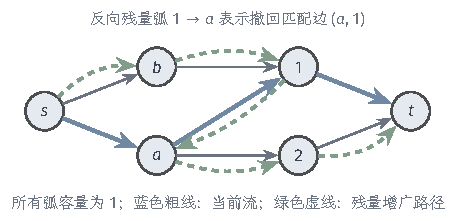
\includegraphics[width=77.093mm]{figures/01-basic-mathematics/04-graphs/tikz/c3-match-flow-network/figure.pdf}
  \caption{图~\ref{fig:graph-opt-match-maximal-maximum}的二部图对应的单位容量网络。蓝色粗弧是匹配$\{(a,1)\}$对应的流；绿色虚线是一条残量$s$--$t$路径，反向残量弧$1\to a$表示撤回$(a,1)$，去掉$s,t$即交替路径$b,1,a,2$。}
  \label{fig:graph-opt-match-flow-network}
\end{figure}

设$\bm x$对应匹配$M$。残量网络中，弧$s\to u$存在当且仅当$u$自由；左侧顶点只能沿未匹配边走到右侧；右侧顶点$w$若自由就走$w\to t$结束，否则只能沿反向残量弧回到伙伴，相当于准备撤回这条匹配边。去掉两端的$s$与$t$，剩下的路径从左到右走未匹配边、从右到左走匹配边。图~\ref{fig:graph-opt-match-flow-network}中的残量路径就是$b,1,a,2$：$b$要任务$1$，请$a$改做任务$2$。

一般地，给定匹配$M$，边交替地不属于$M$与属于$M$的路径称为\term{交替路径}（alternating path）；两个端点都自由的交替路径称为关于$M$的增广路径。在二部图中，增广路径的一端是自由左侧顶点，另一端是自由右侧顶点；首尾两条边都不在$M$中，未匹配边比匹配边多一条。

\begin{lemma}[沿增广路径翻转]
\label{lem:graph-opt-match-flip}
设$P$是关于匹配$M$的增广路径。把$P$上属于$M$的边移出、不属于$M$的边加入，得到的边集$M'$仍是匹配，且$|M'|=|M|+1$。
\end{lemma}

\begin{proof}
$P$外的顶点不受影响。$P$的内部顶点恰关联$P$上一条匹配边和一条未匹配边，且唯一的匹配边就在$P$上，翻转后两者互换，仍恰有一个伙伴。$P$的两个端点原来自由，翻转后各得到一个伙伴。所以$M'$中没有两条边共享端点。$P$上未匹配边比匹配边多一条，故$|M'|=|M|+1$。
\end{proof}

沿残量路径增广一单位，正是沿对应的增广路径翻转，所以最大流的最优性判据可以搬到匹配上。

\begin{theorem}[增广路径判据]
\label{thm:graph-opt-match-augmenting}
二部图中的匹配$M$是最大匹配，当且仅当不存在关于$M$的增广路径。
\end{theorem}

\begin{proof}
若存在增广路径，由引理~\ref{lem:graph-opt-match-flip}可得更大的匹配。反过来，设不存在增广路径，令$\bm x$是$M$对应的流。由上面的对应，残量网络中没有$s$--$t$路径，由定理~\ref{thm:graph-opt-augmenting-path}，$\bm x$是最大流。任何匹配$M''$都对应一个流值为$|M''|$的流，所以$|M''|\leq|M|$。
\end{proof}

这个判据比“不能再加边”强。图~\ref{fig:graph-opt-match-maximal-maximum}(a)中，$\{(a,1)\}$已不能直接加边，却有增广路径$b,1,a,2$；翻转后得到最大匹配$\{(a,2),(b,1)\}$。整体重排能多配一对，是因为中间的顶点只换伙伴，两端的自由顶点各得到一个伙伴。

\subsection{匈牙利算法}
\label{sec:graph-opt-match-algorithm}

定理~\ref{thm:graph-opt-match-augmenting}提示了一种算法：找到增广路径就翻转，找不到就停止。中文教学常把逐个左侧顶点用深度优先搜索找增广路径的做法称为\term{匈牙利算法}（Hungarian algorithm），也称Kuhn算法；英文文献中的Hungarian algorithm通常指第~\ref{sec:graph-assignment}节处理成本的指派算法。它沿用残量增广的思想，但只维护配对关系。

\subsubsection{主要思想}

把图~\ref{fig:graph-opt-match-maximal-maximum}中的$a,b$看成员工甲、乙：甲能做任务$1$和$2$，乙只会任务$1$。甲先接下任务$1$；轮到乙时任务$1$已有人负责，直接找空任务失败。换个问法：先问甲能否改做别的。任务$2$空着，甲改做$2$，空出的任务$1$交给乙。想要的任务已有负责人时，不放弃也不抢走，先替原负责人找去处。

这次调整可以写成$\text{乙}\to1\to\text{甲}\to2$：候选分配、已有分配、候选分配依次交替，终点任务$2$空闲。找到空任务后再逆序落实：甲改做$2$，乙接手$1$。

再增加一名员工和一项任务：甲会$1,2$，乙会$2,3$，丙只会$1$，当前已有甲—1、乙—2。丙想要任务$1$，就请甲另找；甲想要任务$2$，又请乙另找；乙找到空任务$3$。沿$\text{丙}\to1\to\text{甲}\to2\to\text{乙}\to3$连续让位，三人都有了任务，如图~\ref{fig:graph-opt-match-augment}。替甲、替乙找去处是同一个问题，所以可以递归：为某人找任务时，逐个询问他会的任务，任务空着就成功，否则递归地为该任务的负责人另找任务。

\begin{figure}[!htb]
  \centering
  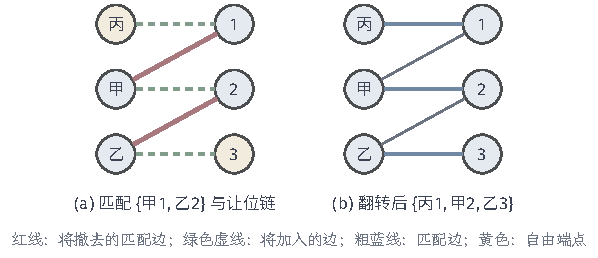
\includegraphics[width=101.279mm]{figures/01-basic-mathematics/04-graphs/tikz/c3-match-augment/figure.pdf}
  \caption{三人三任务的让位链。(a)当前匹配为甲—1、乙—2，丙与任务$3$自由（黄色），让位链交替经过将加入的边（绿色虚线）与将撤去的匹配边（红线）；(b)翻转后配对数由$2$增为$3$。}
  \label{fig:graph-opt-match-augment}
\end{figure}

把员工和任务还原为左右顶点，成功的让位链就是从自由左侧顶点到自由右侧顶点的增广路径，逆序落实就是引理~\ref{lem:graph-opt-match-flip}的翻转；某个分支失败，原负责人找不到去处，原匹配应保持不变。与最大流归约相比，这里只用伙伴数组，省去源汇、容量和残量弧，但这只减少状态，不保证渐近界更优\scite{math-graph-sedgewick-bipartite-matching}。

\subsubsection{算法流程}

\paragraph{算法状态与初始化}
手工调整要记两件事：谁现在负责哪项任务；本轮哪些任务已经问过。前者成功改配后改变并跨轮保留；后者只属于本轮，重问只会重复同样的结果。邻接表在运行前给定、运行中不变，不算状态。取较小的一侧作为左侧，记其顶点数为$p$，算法维护：
\begin{itemize}
  \item 伙伴数组$\mu_L(u)$与$\mu_R(w)$：左右顶点的当前伙伴，初值全为空，即$M=\varnothing$；
  \item 访问时间戳$\tau(w)$：右侧顶点$w$最近一次被询问时的轮次，初值全为$0$；
  \item 当前轮次$k$：初值为$0$。
\end{itemize}
每处理一个左侧顶点就令$k\gets k+1$，本轮已问过的恰是$\tau(w)=k$的右侧顶点，旧标记自动失效，不必清空。新处理的左侧顶点从未被询问，总是自由的。

\paragraph{搜索与改配}
为左侧顶点$u$寻找增广路径的过程$\mathrm{Try}(u)$按邻接表扫描$u$的邻居$w$：
\begin{itemize}
  \item 若$\tau(w)=k$：本轮已问过，跳过；
  \item 否则令$\tau(w)\gets k$。若$w$自由，或递归调用$\mathrm{Try}(\mu_R(w))$成功，就令$\mu_R(w)\gets u$、$\mu_L(u)\gets w$，返回成功；否则继续扫描下一个邻居。
\end{itemize}
邻居扫描完仍未成功，返回失败。伙伴只在成功分支上改写，所以整轮失败时原匹配完整保留。外层对每个左侧顶点依次调用$\mathrm{Try}$，处理完即停止。

成功时改写从链尾向链头逐层进行：内层先为靠后的员工记下新任务，外层才把前一项任务改记给新负责人。两步之间，该任务在$\mu_R$中仍记着原负责人，而原负责人在$\mu_L$中已记着新任务；回到链头时两数组重新一致，所以匹配只在一轮结束后对外使用。

\begin{algorithm}[匈牙利算法]
\label{alg:graph-opt-augmenting-matching}
输入：二部图的左侧邻接表，左侧为较小的一侧。输出：最大匹配的伙伴数组。
\begin{enumerate}
  \item 令全部伙伴为空，全部$\tau(w)=0$，$k=0$。
  \item 对左侧顶点$u$依次执行：令$k\gets k+1$，调用$\mathrm{Try}(u)$。
  \item 输出$\mu_L,\mu_R$。
\end{enumerate}
过程$\mathrm{Try}(u)$：对$u$的每个邻居$w$，若$\tau(w)=k$则跳过；否则令$\tau(w)\gets k$，若$\mu_R(w)$为空或$\mathrm{Try}(\mu_R(w))$返回成功，令$\mu_R(w)\gets u$、$\mu_L(u)\gets w$并返回成功。全部邻居扫描完后返回失败。
\end{algorithm}

\paragraph{运行示例}
表~\ref{tab:graph-opt-match-trace}按“询问—递归—成功返回—改配”逐行列出两个例子，邻居按编号读取。三任务例多递归一层，做法不变；其下半第$3$行$\mu_R$把任务$2,3$都记在乙名下，正是上述暂时不对应。

\begin{table*}[!htb]
  \centering\small
  \caption{匈牙利算法的运行。上半为两任务例，下半为三任务例的第$3$轮（前两轮已得甲—1、乙—2）。$\tau$与$\mu_R$按任务编号列出，“—”表示空。}
  \label{tab:graph-opt-match-trace}
  \begin{tabular}{@{}cllll@{}}
    \toprule
    轮 & 调用栈 & 动作 & $\tau$ & $\mu_R$ \\
    \midrule
    $1$ & 甲 & 问$1$：空闲，记甲—1，成功 & $(1,0)$ & (甲,—) \\
    $2$ & 乙 & 问$1$：甲负责，为甲递归 & $(2,0)$ & (甲,—) \\
    $2$ & 乙，甲 & 跳过$1$；问$2$：空闲，记甲—2，成功 & $(2,2)$ & (甲,甲) \\
    $2$ & 乙 & 收到成功，记乙—1 & $(2,2)$ & (乙,甲) \\
    \midrule
    $3$ & 丙 & 问$1$：甲负责，为甲递归 & $(3,2,0)$ & (甲,乙,—) \\
    $3$ & 丙，甲 & 跳过$1$；问$2$：乙负责，为乙递归 & $(3,3,0)$ & (甲,乙,—) \\
    $3$ & 丙，甲，乙 & 跳过$2$；问$3$：空闲，记乙—3，成功 & $(3,3,3)$ & (甲,乙,乙) \\
    $3$ & 丙，甲 & 收到成功，记甲—2 & $(3,3,3)$ & (甲,甲,乙) \\
    $3$ & 丙 & 收到成功，记丙—1 & $(3,3,3)$ & (丙,甲,乙) \\
    \bottomrule
  \end{tabular}
\end{table*}

失败的搜索要保留原匹配。在三任务例中删去允许边甲—2，前两轮仍得到甲—1、乙—2，第$3$轮为：
\begin{itemize}
  \item 丙询问任务$1$，令$\tau(1)=3$，任务$1$由甲负责，为甲递归；
  \item 甲只会任务$1$，而它本轮已问过，甲的搜索失败，不改任何记录；
  \item 丙再无别的任务可问，整轮失败。
\end{itemize}
伙伴数组仍是甲—1、乙—2。若丙询问时就先撤去甲—1，甲、丙都将没有任务，匹配反而少一对。

\subsubsection{正确性与复杂度}

在三人让位链上数配对：甲、乙只换了任务，丙和任务$3$各得到伙伴，恰好多$1$对，一般情形即引理~\ref{lem:graph-opt-match-flip}。还需说明搜索失败时当前匹配已不能改进。

\begin{theorem}[匈牙利算法的正确性]
设左侧顶点按$u_1,\ldots,u_p$的顺序处理，$\mathcal G_k$为由$u_1,\ldots,u_k$与全部右侧顶点导出的子图。处理完$u_k$后，伙伴数组给出$\mathcal G_k$的一个最大匹配；特别地，算法输出$\mathcal G$的最大匹配。
\end{theorem}

\begin{proof}
对$k$归纳，$k=0$时匹配为空，结论成立。设处理$u_k$前的匹配$M$是$\mathcal G_{k-1}$的最大匹配，$u_k$是自由顶点。$\mathcal G_k$只比$\mathcal G_{k-1}$多一个顶点$u_k$，任何匹配中至多一条边含$u_k$，所以$\mathcal G_k$的最大匹配数至多比$\mathcal G_{k-1}$的多$1$。

若$\mathrm{Try}(u_k)$成功，递归链依次经过$u_k$、右侧顶点$w_1$、$w_1$的伙伴、右侧顶点$w_2$、……，止于一个自由右侧顶点。本轮每个右侧顶点至多问一次，链上的左侧顶点互不相同，所以这条链是增广路径，逐层改写就是翻转。由引理~\ref{lem:graph-opt-match-flip}，新匹配有$|M|+1$条边，达到上述上界，是$\mathcal G_k$的最大匹配。

若$\mathrm{Try}(u_k)$失败，伙伴数组未变。记本轮被询问过的右侧顶点集为$R^*$，$L^*$由$u_k$与$R^*$中顶点的伙伴组成。被询问的右侧顶点都不自由，本轮对其伙伴调用过$\mathrm{Try}$，失败的$\mathrm{Try}$扫描了全部邻居，所以$L^*$中每个顶点的邻居都在$R^*$中。于是从$u_k$出发的交替路径始终留在$L^*\cup R^*$中，到不了自由右侧顶点。假如$M$不是$\mathcal G_k$的最大匹配，由定理~\ref{thm:graph-opt-match-augmenting}存在增广路径$P$。$P$的内部顶点都已匹配，不会是自由的$u_k$；若$u_k$也不是$P$的端点，$P$就整条位于$\mathcal G_{k-1}$中，与$M$在$\mathcal G_{k-1}$中最大矛盾。所以$P$从$u_k$出发，而这刚被排除。故$M$仍是$\mathcal G_k$的最大匹配。
\end{proof}

同一轮中每个右侧顶点至多被询问一次，每个左侧顶点至多调用一次$\mathrm{Try}$（它是$u_k$，或某个被询问右侧顶点的伙伴），所以每条允许边至多扫描一次，一轮为$O(1+m)$。$p$轮共$O(p+pm)$，加上伙伴数组与时间戳的初始化$O(n)$，总时间为$O(n+pm)$；邻接表、伙伴数组与时间戳共占$O(n+m)$空间。若每轮清空访问数组，另需$O(|R|)$；用邻接矩阵时每次扫描要读整行，也须另算代价。

\subsubsection{分层增广的进一步改进}
\label{sec:graph-opt-hopcroft-karp}

逐点搜索每轮至多找到一条增广路径。Hopcroft--Karp算法把第~\ref{sec:graph-opt-dinic}节Dinic算法的分层思想用到单位容量网络上，每个阶段做两步：
\begin{itemize}
  \item 分层：从全部自由左侧顶点同时沿交替路径做广度优先遍历，求出最短增广路径长度与各顶点层号；
  \item 增广：只沿层号逐层加一的边做深度优先搜索，找出一组极大的、顶点互不相交的最短增广路径，一起翻转。
\end{itemize}
这组路径就是分层残量网络中的阻塞流（定义~\ref{def:graph-opt-blocking-flow}），与Dinic算法同理，每个阶段之后最短增广路径的长度严格增加。阶段数很少，理由简述如下：$\sqrt n$个阶段之后，最短增广路径已有超过$2\sqrt n$条边；当前匹配与任一最大匹配的差可以分解为顶点互不相交的增广路径，每条都占去超过$\sqrt n$个顶点，所以至多还差$\sqrt n$条，至多再需$\sqrt n$个阶段。每阶段为$O(m)$，主计算为$O(m\sqrt n)$；孤立顶点不在任何增广路径上，先用$O(n)$时间删去，总时间写作$O(n+m\sqrt n)$\scite{math-graph-sedgewick-hopcroft-karp}。这个界不适用于前面逐点搜索的实现。

\subsection{结果检验}
\label{sec:graph-opt-match-analysis}

先确认可行性：所选边都是允许边，两两没有公共端点，再重数边数；伙伴数组还应两两对应，即$\mu_L(u)=w$当且仅当$\mu_R(w)=u$。

最大性另需证据：可以从全部自由左侧顶点重做一次交替搜索，确认到不了自由右侧顶点；更独立的证据是单位容量网络中容量等于$|M|$的割。令$Z$为从自由左侧顶点沿交替路径能到达的顶点集，若其中没有自由右侧顶点，取源侧$S=\{s\}\cup Z$。这时$Z$中左侧顶点的邻居都在$Z$中，$Z$中的右侧顶点都已匹配且伙伴也在$Z$中，所以跨出$S$的弧只有$s\to u$（$u\in L\setminus Z$）与$w\to t$（$w\in R\cap Z$）。对每条匹配边$(u,w)$，$u\in Z$时恰有$w\to t$跨出，$u\notin Z$时$w\notin Z$，恰有$s\to u$跨出；自由顶点不贡献跨出的弧。故割容量为$|M|$，由引理~\ref{lem:graph-opt-weak-duality}，$M$最大。在删去甲—2的例子中，$Z=\{\text{丙},1,\text{甲}\}$，跨出$S$的弧是$s\to\text{乙}$与$1\to t$，割容量为$2$，等于匹配的边数。

不能因为自由顶点之间没有允许边就宣布最大：图~\ref{fig:graph-opt-match-maximal-maximum}(a)中自由的$b$与$2$不相邻，却仍有增广路径。

完整配对可能有多种，数量无法区分优劣。第~\ref{sec:graph-assignment}节给配对加上成本，选出总成本最小的完整配对。
